\section{Lecture 3}
\subsection{Electrical properties of a cell}
\subsubsection{General ohmic model}
\begin{tabular}{p{4cm}p{15cm}}
Circuit representation of biological membrane	& 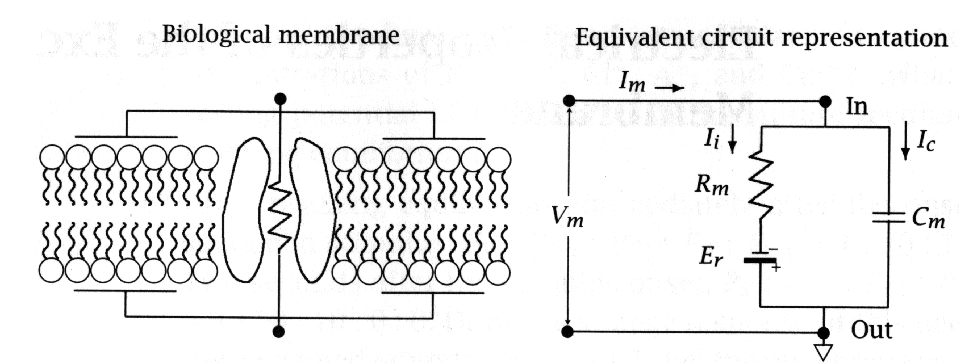
\includegraphics[width = 14cm]{neuroinf_biomembrane_as_circuit.png}\\
Capacitance $(C_m, V_m)$	& The capacitance is determined by the properties of the lipid bilayer (polar heads are conducting, apolar tails are isolating (dielectricum)) and is \textbf{fixed}.\\
Conductance $(g_m)$	& The conductance represents the various channels (carrier protein, channel protein, sodium-potassium pump), whose permabilities are \textbf{variable}. The conductance is of course inverse to the resistance $R_m$\\
Battery $(E_r)$		& The battery represents the resting potential arising by persistent concentration gradients. The resting potential is \textbf{fixed}.\\
Current $(I_m)$		& $I_m = C_m \frac{dV_m}{dt} + \frac{V_m-E_r}{R_m}$. Unless there is a arbitrary current from outside (for experiments), $I_m = 0$
\end{tabular}
\subsubsection{Ohmic model applied on neuron}
\begin{longtable}{p{4cm}p{15cm}}
Total current	& \begin{tabular}[t]{ll}
             	  $I_m$ 	& $= I_C + I_K + I_{Na} + I_{Cl}\quad I_m = $external current source\\
				& $= C_m \frac{dV}{dt} + g_k(V-E_k) + g_{Na}(V-E_{Na}) + g_{Cl}(V-E_{Cl})$
             	  \end{tabular}\\
Resting potential ($I_m = 0, \frac{dV}{dt} = 0$)	& $\boxed{V_{rest} = V = \frac{g_kE_k + g_{Na}E_{Na} + g_{Cl}E_{Cl}}{g_k + g_{Na} + g_{Cl}}}$\\
				& This is the GHK voltage equation in electrical terms.\\
Typical membrane parameters	& \begin{tabular}[t]{l|ll}
								& Independent of geometry	& for cylinder\\\hline
					    Diameter		& -				& $a = 20 \mu m$\\
					    Capacitance		& 1 $\mu F / cm^2$		& $c_m = C_m 2\pi a L \approx 10$ pF\\
					    Membrane Resistance	& $R_m = 10 k\Omega cm^2$	& $r_m = \frac{R_m}{2\pi a L} \approx 1 $G $\Omega$\\
					    Axial resistance	& $R_a = 100 \Omega cm$		& $r_a = \frac{R_a}{a^2 \pi}$\\
					    Time constant	& -				& $\tau = c_m r_m \approx 10$ ms
					  \end{tabular}\\
Current loss in axon	& \begin{tabular}[t]{p{14cm}}
			  There is an exponential decay of voltage due to leakages to the extracellular area. This decay can be modeled with the cable equation.\\
			  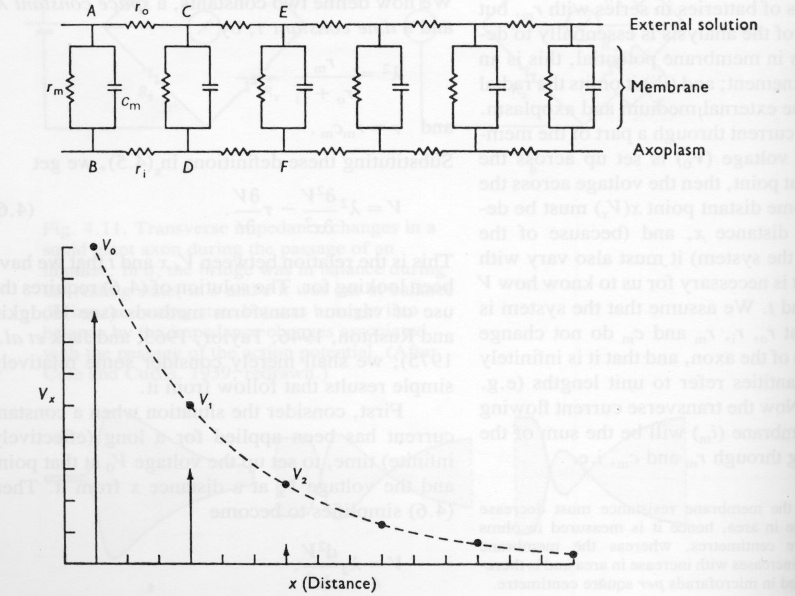
\includegraphics[width = 10cm]{neuroinf_voltagelossaxon.png}
			  \end{tabular}\\
Cable equation		& \begin{tabular}[t]{l}
			   $\boxed{\tau \left(\frac{\partial v}{\partial t} \right) = \lambda^2 \left( \frac{\partial^2v}{\partial x^2} \right) - v + r_m i_e}$\\
			   $\lambda = \sqrt{\frac{r_m}{r_a}} = \sqrt{\frac{a R_m}{2 R_a}}\qquad v = V-V_{rest}$\\
			   $i_e$: injected current\\
			   $r_m$: membrane resistance (geometry dependent)\\
			   $r_a$: axial resistance (geometry dependent)\\
			   $\lambda$: space constant. For $x=\lambda$, the voltage has decayed about an $e$-fold.
			  \end{tabular}\\
Stationary solution	& $\boxed{v(x) = \left( \frac{i_e R_{\lambda}}{2} \right) e^{-|x| / \lambda}}$\\
Remarks on $\lambda$& \begin{itemize}
				\item The bigger $\lambda$, the better (in terms of voltage transfer)
				\item The bigger the diameter, the bigger $\lambda$
				\item The bigger the membrane resistance, the bigger $\lambda$
				\item For a human membrane, $\lambda \approx 0.6$ mm
                           \end{itemize}
\end{longtable}
\subsection{Basic formulae}
\begin{tabular}{p{4cm}p{15cm}}
Ohm's Law	& $U = R \cdot I$\\
Capacitance	& $C = \frac{q}{U}$\\
Current and Capacitance	& $I = C \frac{dV}{dt}$\\
Conductivity	& $g = \frac{1}{R}$\\
Charging of a capacitor	& $\frac{I_{inj}}{g}(1-e^{-t/\tau}) + E$\\
Kirchhoff Current Law	& Inflow = Outflow at a node\\
Kirchhoff Voltage Law	& In every circuit, the sum of the voltages must be zero
\end{tabular}